%------------------------------------------%
% \subsection{O Papel do Software na Ciência}
% \label{sec:software:ciencia}
% \subsection{A Importância do Software de Pesquisa}
%------------------------------------------%
\section{Software na Ciência} \label{sec:software:ciencia}

Na Ciência moderna, os dados de pesquisa (\textit{research data}) dependem, de modo crescente, do ambiente de software em que foram criados, gerenciados, analisados e apresentados. 
Resultados digitais da pesquisa, como publicações científicas e conjuntos de dados abertos, não podem ser visualizados ou usados sem o software apropriado. 
%Ainda, software usualmente tem um curto ciclo de vida, rapidamente se tornando inútil se não for apropriadamente mantido e sustentado. 

Muitas instituições, grupos e pesquisadores 
%(incluindo o UK’s Software Sustainability Institute \footnote{\url{http://www.software.ac.uk}}) 
reconhecem que todo o software desenvolvido no contexto de uma pesquisa científica deve ser considerado um resultado de pesquisa \cite{jay_software_2021} e que 
a boa prática científica exige que o software mencionado em publicações científicas seja mantido para reprodutibilidade e verificação de resultados científicos.
%
O Manifesto do Código da Ciência (\textit{Science Code Manifesto})\footnote{\url{http://sciencecodemanifesto.org/}} destaca a importância do software usado ou desenvolvido \textit{durante} a pesquisa científica:
\begin{quote}
   ``Software é um produto de pesquisa essencial e o esforço para produzir, manter, adaptar, e fazer a curadoria do código deve ser reconhecido. O Software é parte de outras contribuições científicas vitais além de artigos publicados.''  
\end{quote}

%------------------------------------%

\subsection{Software como Instrumento}

%Software e hardware especializados são usados para a captura, processamento, manipulação, registro, relatório, armazenamento ou recuperação de calibração ou dados de teste. Neste contexto, o software de computador deve estar documentado e adequado para uso.

% Instrumentos científicos contém uma quantidade significativa de software
Software é usado como parte integral de muitos instrumentos científicos, por exemplo, telescópios e microscópios. 
%Instrumento pode ser tanto físico quanto virtual; por exemplo, 
Outras vezes, o próprio software é o instrumento, gerando dados de pesquisa, validando dados de pesquisa, ou testando hipóteses. 
Isto inclui métodos computacionais ou modelos e simulações, por exemplo, modelos climáticos, modelos baseados em agentes em ciências sociais, simulação de hardware, dentre outros \cite{nieuwpoort_defining_2023}.

\subsection{Software como Contribuição Científica}

Software tornou-se parte fundamental de um ecossistema científico que engloba recursos, publicações~\cite{howison2011scientific} e 
possui a particularidade de se relacionar com o sistema econômico de reputação científica, especialmente com o seu modelo de publicações, influenciando e sendo influenciado diretamente pelo impacto de suas publicações \cite{howison2015understanding}.

A Figura~\ref{fig:scientific-reputation-diagram} mostra que a \textit{Pesquisa} conduzida por um ou mais pesquisadores pode gerar \textit{Publicações científicas} com resultados para a área do conhecimento, e também pode produzir \textit{Software} e \textit{Publicação do software}~\cite{howison2015understanding}.
As publicações científicas podem receber \textit{Citações} dos pares, o que contribui para aumentar a \textit{Reputação} acadêmica dos pesquisadores e, eventualmente, retroalimentar o sistema na forma de novos \textit{Recursos} para a pesquisa.

\begin{figure}[tb]
  \center
  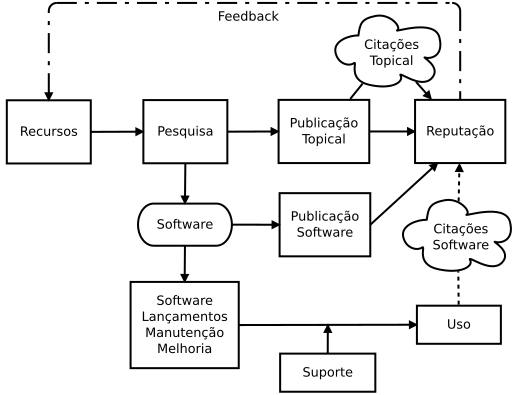
\includegraphics[scale=0.4]{figures/scientific-reputation-diagram.png}
  \caption{Uma visão dos incentivos de reputação num contexto misto entre Ciência e práticas de software de pesquisa.~\cite{howison2011scientific}}
  \label{fig:scientific-reputation-diagram}
\end{figure}

A Figura~\ref{fig:scientific-reputation-diagram} também relaciona  \textit{Software} a \textit{Lançamentos, Manutenção e Melhoria}
que exigem \textit{Suporte} e levam à disponibilização do software para \textit{Uso}.
Entretanto, não há uma ligação direta e explícita entre a publicação do software e eventuais citações ao software. As setas tracejadas sugerem que o \textit{Uso} do software pode gerar citações ao software e que estas podem influenciar de modo diferente (ou mesmo não influenciar) a reputação dos pesquisadores.
Este problema pode ser explicado pela falta de padronização da citação de software e prática frequente de ``citar'' apenas uma URL que leva a um local onde o software pode ser encontrado. 
  
A citação de software permite aos desenvolvedores receber reconhecimento e crédito pelo seu trabalho, além de facilitar a rastreabilidade e replicação dos resultados. Também contribui para a visibilidade e a colaboração na comunidade científica, fortalecendo a sustentabilidade técnica do software. No entanto, a importância do software na pesquisa ainda é subestimada, e o software é tratado como um recurso de apoio ou ferramenta, e não como uma contribuição científica em si. 
%
No ecossistema da Ciência Aberta, o software de pesquisa deve ser citável e reconhecido como uma valiosa contribuição da pesquisa científica, tão importante quanto os artigos publicados, dados e metadados.  No entanto, esforços e incentivos são necessários para que os créditos para o software de pesquisa se tornem mais específicos e rastreáveis na Ciência.

\subsection{\textit{Better Software, Better Research}}

% Artigo ``Better Software, Better Research''~\cite{goble2014better}.
% The continued development of science is partly dependent on improvements in research software. Despite the reliance on software in academia, professional practices for its development too often lag behind those in the commercial sector.

%The pressure on researchers to rapidly publish new results without the need to develop professional quality code results in fragile academic research software, generally not sustainable or usable beyond the lifetime of a given project. As a result, the research community fails to benefit from their research's potential impact fully.

Pesquisadores sofrem uma intensa e constante pressão para publicar novos resultados rapidamente sem a devida cobrança sobre a necessidade de desenvolver código de qualidade. Como consequência, o software desenvolvido durante a pesquisa tende a não ser sustentável ou usável além da duração da pesquisa ou dos recursos que a  financiam, e impede a comunidade científica de aproveitar plenamente o seu potencial impacto em pesquisas futuras.

%\subsection{Histórico} 
Em 2016, inspirada pelo artigo 
\textit{Better Software, Better Research}~\cite{goble2014better}, 
o workshop \textit{Dagstuhl Perspectives}~\cite{goble_et_al:DR:2016:6755} reuniu ativistas, especialistas e interessados em discutir sobre o software produzido no contexto acadêmico e sua qualidade, na perspectiva de grupos de pesquisa que (i)~consomem ou produzem software como saída do processo científico, ou (ii)~consomem ou produzem software como um dos componentes dos métodos de pesquisa.

Dentre os resultados principais e com base em dados sobre o crescimento no uso de software em pesquisas científicas,
o workshop identificou seis áreas no ecossistema de software de pesquisa que merecem atenção: 
\textit{crédito ao software}, tornando-o rastreável nas pesquisas científicas; \textit{herança cultural}, ou preocupação com as implicações das escolhas tecnológicas; \textit{princípios FAIR para software} (discutidos na Seção 3.4.3); \textit{financiamento} de atividades de desenvolvimento e manutenção de software; \textit{políticas e e práticas} para incentivar a colaboração, a transparência e o compartilhamento de conhecimento entre os pesquisadores e instituições; e necessidade de \textit{treinamentos} para pesquisadores e outros atores envolvidos com o desenvolvimento de software para uso na pesquisa.

Sobre treinamentos, o workshop recomendou que os mesmos devem cobrir diversos tópicos relacionados ao desenvolvimento de software e níveis de prática, e que cursos oferecidos por alguns institutos, por exemplo, \textit{Carpentries}, devem ser estimulados e apoiados.
%
Práticas centrais para manutenibilidade do software devem ser apresentadas, incluindo controle de versão, padrões de codificação, revisão de código, programação em par, testes, cobertura de código, integração contínua, refatoração e documentação. 
%
Outros tópicos também devem ser considerados, por exemplo, quão aberto é um software, se é desenvolvido por uma comunidade ou por um indivíduo, quão ativa é a manutenção do software (correção de \textit{bugs} e criação de novas funcionalidades) ou disponibilidade de recursos diversos~\cite{sufi_report_2020}.

%
%A próxima seção apresenta conceitos e atributos do \textit{software de pesquisa} \cite{gruenpeter_morane_2021_5504016} e destaca a sua importância no ecossistema da Ciência Aberta.
